\section{Artículo complementario}
\label{articulo_complementario}


El articulo complementario que se ha estudiado durante la realización de este proyecto tiene por título \textsl{"Quasi-Randomized Path Planning"}, y fue escrito por M. Branicky, S. La Valle, K. Olson y L. Yang.. En el se propone un enfoque distinto a la hora de muestrear el espacio por el que se moverá el robot, pasando a distribuir los nodos de forma cuasi-aleatoria, en vez de hacerse por completo aleatoriamente.
\\

Cuando se trabaja en un espacio de configuraciones con un alto número de variables a considerar, las aproximaciones deterministas clásicas desarrolladas para la planificación de trayectorias dejan de ser aplicables, o son demasiado costosas. Para estos casos, en la década de los 90 se comenzarom a desarrollar enfoques aleatorios. Estos métodos pasaron a ser mas usados que los deterministas por dos motivos:
\begin{enumerate}
\item Permitían resolver un problema con una alta multidimensionalidad sin la necesidad de explorar todas las alternativas.
\item Si se ve el problema como un enemigo a vencer, a menudo se puede evitar la derrota aplicando una estrategia aleatoria, cosa que no ocurre con una determinista. 
\end{enumerate}  

Sin embargo, no es posible conseguir una serie de datos realmente aleatorios, ya que cualquier posible implementación simplemente llevará a una secuencia determinista de números pseudoaleatorios que van a seguir una cierta función de probabilidad. De aquí se sacó la idea de desarrollar un metodo cuasi-aleatorio que permitiese solucionar el problema de la generación de trayectorias de forma más eficaz. 
\\

A la hora de generar la secuencia de muestras pseudo-aleatorias con las que va a trabajar el método aleatorio de planificación, se busca el conjunto de puntos que optimicen el valor de dos parámetros, la discrepancia y la dispersión. La discrepancia para un conjunto P formado por N muestras de d-dimensiones en $[0,1]^{d}$  viene dada por la ecuación 2.1:
\begin{equation}
D_{N}(P) = \sup_{j} |\frac{A(J)}{N}-\mu(J)|
\end{equation} 

Donde J es cualquier subconjunto n-rectangular perteneciente a $[0,1]^{d}$, $\mu(J)$ es su medida n-dimensional y A(J) es el número de puntos que pertenecen a la unión entre P y J. En cuanto a la dispersión, hace referencia a la máxima distancia a la que cada punto de un conjunto puede estar respecto al punto mas cercano perteneciente a la misma secuencia. Por lo general, los conjuntos de puntos que presentan una baja discrepancia también poseerán una baja dispersión.
\\

Se desarrollaron cuatro distintos conjuntos de muestras:
\begin{enumerate}
\item Cuadrículas: Consiste en la cuantificación uniforme de cada uno de los ejes de coordenadas.
\item Enrejado: Generalización que mantiene la estructura de una cuadrícula, pero es generado por un conjunto de bases generalmente no ortogonales que buscan obtener una baja discrepancia.
\item Método cerrado: No requiere una estructura de vecindad para las muestras, cuyo número debe ser conocido a priori.
\item Método abierto: No es necesario conocer a priori el número de muestras. Por lo general, se obtiene una discrepancia más alta entre las muestras que con el método cerrado 
\end{enumerate}

El primer grupo es un subconjunto del segundo, que a su vez es un subconjunto del tercero. Para probar los resultados que ofrece el uso del método abierto y el cerrado desarrollaron una variante del algoritmo Probabilistic Road Map (de ahora en adelante PRM), mientras que para probar los otros dos conjuntos optaron por una variación del Lazy PRM.
\\

El algoritmo PRM y sus variantes se pueden dividir en dos fases. La primera consisitiría en la generación aleatoria de nodos dentro del mapa con el que se está trabajando. Estos nodos se conectan entre sí para crear un grafo, siempre evitando generar nodos o conexiones encima de obstáculos. Una vez obtenido dicho grafo, la segunda fase consiste en encontrar el camino mas corto entre el punto inicial y el final, a través de las distintas conexiones que conforman el grafo.
\\

En cuanto al Lazy PRM, sigue la misma estructura que el PRM clásico, con una diferencia. Durante la primera fase, al generar el grafo, no se tienen en cuenta los obstáculos al distribuir los nodos y crear las conexiones entre ellos. Después, se usa un algoritmo para encontrar el camino a través del grafo (en este caso se ha usado el A*) y se genera una trayectoria. Por último, se comprueba si alguno de los tramos del camino colisiona con un obstáculo. Si esto ocurre, se elimina la conexión o el nodo que colisione y se vuelve a buscar el camino. Esto se repite hasta que se encuentre una solución factible. Por lo general, la comprobación de colisiones es bastante costosa computacionalmente, por lo que empleando este método se puede reducir el tiempo de cálculo en entornos con una gran cantidad de nodos y de obstáculos.  
\\

\begin{figure}[h]
		\centering
        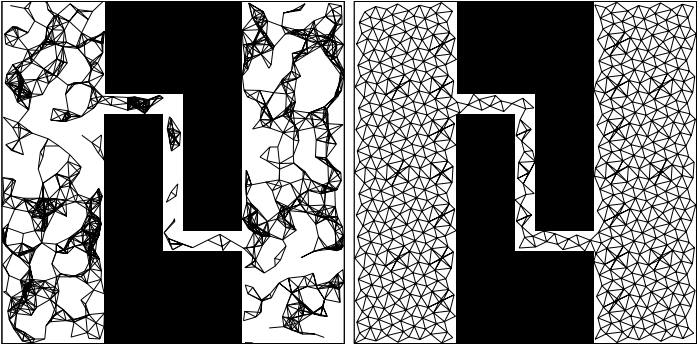
\includegraphics[width=0.35\textwidth]{images/PRM_y_Q-PRM.png}
        \caption{Comparación entre PRM y Q-PRM}
        \label{fig:comparacion_algoritmos}
\end{figure} 

En la figura \ref{fig:comparacion_algoritmos} se puede observar el resultado de aplicar un muestreo aleatorio del espacio libre para generar los nodos. Al coger puntos al azar se da lugar a que existan grandes regiones del espacio en la que no existan nodos, mientras que puede haber otras con un mayor numero de puntos de los que son realmente necesarios. Como consecuencia directa de esto, en casos donde el espacio sea limitado, como puede ser mapas con una gran densidad de obstáculos o pasillos estrechos, podría llegar a no encontrarse un camino, al no presentar nodos lo suficientemente cerca como para que exista una conexión entre ellos.
\\

Para tratar de solucionar esto, se han desarrollado conjuntos deterministas de puntos, con los que se trata de explorar de manera mas efectiva el espacio libre, además de reducir la discrepancia entre puntos. En conccreto, en este paper se utilizan tres distinos tipos de datos de entrada, conocidos como puntos de Hammersley, puntos de Halton y puntos de Faure. Se hablará mas en profundidad acerca de estos conjuntos en la sección 4.2.
\\

Con esto se consigue solucionar algunos de los problemas que presentan las aproximaciones totalmente aleatorias sin que desaparezcan las ventajas que estos métodos presentan frente a los métodos deterministas clásicos.
\\
\\